\apendice{Especificación de Requisitos}

\section{Introducción}

Una parte imprescindible para llevar a cabo cualquier proyecto de \textit{software} son los requisitos, que definirán el comportamiento esperado por el producto final. Una vez especificados estos se podrá proceder al desarrollo del proyecto, utilizando como guía la definición de requisitos realizada.

La especificación de requisitos abarcan tanto las funciones de las que debe de ser capaz el producto, los conocidos como requisitos funcionales; como de comportamiento de este y otras características no relacionadas a sus funciones, los requisitos no funcionales.
%Una muestra de cómo podría ser una tabla de casos de uso:
%
%% Caso de Uso 1 -> Consultar Experimentos.
%\begin{table}[p]
%	\centering
%	\begin{tabularx}{\linewidth}{ p{0.21\columnwidth} p{0.71\columnwidth} }
%		\toprule
%		\textbf{CU-1}    & \textbf{Ejemplo de caso de uso}\\
%		\toprule
%		\textbf{Versión}              & 1.0    \\
%		\textbf{Autor}                & Alumno \\
%		\textbf{Requisitos asociados} & RF-xx, RF-xx \\
%		\textbf{Descripción}          & La descripción del CU \\
%		\textbf{Precondición}         & Precondiciones (podría haber más de una) \\
%		\textbf{Acciones}             &
%		\begin{enumerate}
%			\def\labelenumi{\arabic{enumi}.}
%			\tightlist
%			\item Pasos del CU
%			\item Pasos del CU (añadir tantos como sean necesarios)
%		\end{enumerate}\\
%		\textbf{Postcondición}        & Postcondiciones (podría haber más de una) \\
%		\textbf{Excepciones}          & Excepciones \\
%		\textbf{Importancia}          & Alta o Media o Baja... \\
%		\bottomrule
%	\end{tabularx}
%	\caption{CU-1 Nombre del caso de uso.}
%\end{table}

\section{Objetivos generales}

Los objetivos que se buscan alcanzar con este proyecto son los siguientes:

\begin{enumerate}
	\item Obtención de ubicaciones comerciales de distintas ciudades mediante el uso de peticiones a la API de geolocalización de \textit{OpenStreetMap}.
	
	\item Almacenamiento de dichas ubicaciones en una base de datos no relacional orientada a grafos de Neo4j.
	
	\item Obtención de las relaciones de interacción entre las distintas categorías comerciales, así como de los coeficientes de atracción y repulsión que nos proporcionan la aplicación de distintos métodos.
	
	\item Obtención de índices de calidad en base a los anteriores coeficientes de interacción que nos permitan estimar la adecuación de un establecimiento comercial a
	su ubicación, tanto a su categoría como a otras.
	
	\item Uso tanto individual como combinado (mediante modelos de \textit{machine learning}) de los distintos índices de calidad para hacer recomendaciones de ubicaciones comerciales
	
	\item Integración de datos de distintas ciudades, realizando así transferencia de conocimiento de unas ciudades a otras usando modelos de \textit{machine learning}.
	
	\item Creación de una aplicación web que permita a los usuarios de la herramienta obtener recomendaciones fácilmente mediante los índices de calidad y modelos obtenidos.
	
	El producto final constituirá un sistema de recomendación de categorías comerciales y ubicaciones de forma que se maximicen los beneficios y el rendimiento de hipotéticos negocios en las ubicaciones dadas.
	
	En cuanto a las herramientas a utilizar cabe destacar el uso de Neo4j, una base de datos no relacional que pertenece a un nuevo paradigma, la orientación a grafos. Su aprendizaje y correcto uso será parte crucial del proyecto.
\end{enumerate}

\section{Catalogo de requisitos}

Dados los objetivos del proyecto, extraemos los siguientes requisitos:

\subsection{Requisitos funcionales}

Los requisitos funcionales son aquellos que definen el comportamiento esperado por la aplicación. Nuestro trabajo recoge los siguientes:

\begin{itemize}
	\item \textbf{RF1 - Navegación de Usuarios}
		\begin{itemize}
  			\item \textbf{RF1.1}: El usuario puede navegar por la página web.
			 Puede volver a la página de inicio desde el icono en la esquina superior izquierda.
			\item \textbf{RF1.2}: Acceder a las secciones disponibles desde la barra de navegación superior.
			\item \textbf{RF1.3}:Gestionar la sesión desde el menú desplegable en la esquina superior derecha.
		\end{itemize}
	\item \textbf{RF2 - Búsqueda de Establecimientos}
	\begin{itemize}
		\item \textbf{RF2.1}: El usuario puede buscar establecimientos por ciudad y categoría.
	\end{itemize}
	\item \textbf{RF3 - Interacción con el Mapa}
		\begin{itemize}
			\item \textbf{RF3.1}: La aplicación contará con un mapa donde se mostrarán las ubicaciones registradas.
			\item \textbf{RF3.2}: El usuario puede seleccionar ubicaciones registradas.
			\item \textbf{RF3.3}: El usuario puede seleccionar ubicaciones no registradas previamente mediante la introducción de coordenadas.
			\item \textbf{RF3.4}: Los marcadores seleccionados se mantendrán en el mapa entre búsquedas de categorías.
			\item \textbf{RF3.5}: La aplicación debe de contar con un botón para borrar todas las ubicaciones seleccionadas en el mapa.
			\item \textbf{RF3.6}: Los marcadores deben mostrar detalles al pasar el cursor sobre ellos.
			\item \textbf{RF3.7}: Los marcadores mostrados deben de estar diferenciados entre seleccionados, no seleccionados y marcadores de coordenadas.
			\item \textbf{RF3.8}: Las ubicaciones seleccionadas deben de ser identificables y fácilmente reconocibles en las pantallas de recomendación.
		\end{itemize}
	\item \textbf{RF4 - Recomendaciones de Categorías Comerciales}
	\begin{itemize}
		\item \textbf{RF4.1}: El usuario registrado puede obtener recomendaciones de categorías a nivel local.
		\item \textbf{RF4.2}: El usuario registrado puede obtener recomendaciones de categorías utilizando transferencia de información de otras ciudades.
		\item \textbf{RF4.3}: El usuario podrá elegir el método para recibir estas recomendaciones.
		\item \textbf{RF4.4}: Las recomendaciones se mostrarán como una selección de las categorías más adecuadas para cada ubicación seleccionada.
	\end{itemize}
	\item \textbf{RF5 - Recomendaciones de Ubicaciones}
	\begin{itemize}
		\item \textbf{RF5.1}: El usuario registrado puede obtener recomendaciones de ubicaciones a nivel local.
		\item \textbf{RF5.2}: El usuario registrado puede obtener recomendaciones de ubicaciones utilizando transferencia de información de otras ciudades.
		\item \textbf{RF5.3}: El usuario podrá elegir para qué categoría comercial obtener las recomendaciones.
		\item \textbf{RF5.4}: El usuario podrá elegir qué método emplear para recibir estas recomendaciones.
		\item  \textbf{RF5.5}: Las recomendaciones se mostrarán como un \textit{ranking} de las ubicaciones ordenadas en orden descendente en función de la adecuación de cada ubicación para la categoría seleccionada.
		
	\end{itemize}
	
	\item \textbf{RF6 - Red de Categorías}
	\begin{itemize}
		\item \textbf{RF6.1}: La aplicación debe poder generar una visualización en forma de grafo de la red de interacción entre categorías de cada ciudad.
		\item \textbf{RF6.2}: El usuario podrá elegir de qué ciudad se generará la red de categorías.
		\item \textbf{RF6.3}: Los nodos de cada categoría deben diferenciarse con respecto al resto.
		\item \textbf{RF6.4}: El usuario podrá aplicar un filtro en base al grado de los nodos.
		\item \textbf{RF6.5}: El usuario podrá aplicar un filtro en base a la categoría de los nodos.
	\end{itemize}
	
	\item \textbf{RF7 - Gestión de Usuarios}
	\begin{itemize}
		\item \textbf{RF7.1}: El usuario puede registrarse proporcionando nombre de usuario, nombre, apellidos, correo electrónico y contraseña.
		\item \textbf{RF7.2}: El usuario registrado puede iniciar sesión utilizando su nombre de usuario y contraseña.
		\item \textbf{RF7.3}: El usuario registrado puede cerrar sesión en caso de haberla iniciado previamente.
	\end{itemize}
	
\end{itemize}

\subsection{Requisitos no funcionales}
Los requisitos no funcionales se corresponden con aquellos que no especifican el funcionamiento de la aplicación. Estos definen cómo debe de ser el comportamiento del producto en algunas situaciones o ámbitos.

Nuestra aplicación cuenta con los siguientes:

\begin{itemize}
	\item \textbf{RNF1 - Seguridad}
		\begin{itemize}
			\item \textbf{RNF1.1}: Las contraseñas deben guardarse cifradas en la base de datos.
			\item \textbf{RNF1.2}: Las contraseñas de los usuarios deben de cumplir unas restricciones de longitud.
		\end{itemize}
	\item \textbf{RNF2 - Velocidad de respuesta}
			\begin{itemize}
				\item \textbf{RNF2.1}: La velocidad de carga de ubicaciones debe de ser rápida.
				\item \textbf{RNF2.2}: La velocidad de obtención de recomendaciones debe de ser rápida.
			\end{itemize}
	\item \textbf{RNF3 - Compatibilidad}
		\begin{itemize}
			\item \textbf{RNF3.1}: La aplicación web debe de ser compatible con las últimas versiones de los navegadores.
			\item \textbf{RNF3.2}: La aplicación web debe de ser compatible con HTML5 y CSS3.
		\end{itemize}
	\item \textbf{RNF4 - Usabilidad}
		\begin{itemize}
			\item \textbf{RNF4.1}: La selección de ubicaciones debe de ser cómoda y fácil de realizar.
			
		\end{itemize}
\end{itemize}
%\begin{itemize}
%	\item \textbf{RF-1. Extracción de datos:} La aplicación debe de ser capaz de extraer datos de ubicaciones comerciales.
%		\begin{itemize}
%			\item \textbf{RF-1.1. Extracción de ubicaciones de determinada categoría:} La aplicación debe de ser capaz de extraer ubicaciones con cietegoría asociada.
%			\item \textbf{RF-1.2.Extracción de ubicaciones de rta caciudades:} La aplicación debe permitir extraer ubicaciones de determinados núcleos urbanos.
%		\end{itemize}
%	\item \textbf{RF-2. Almacenamiento de datos:} La aplicación debe guardar los datos obtenidos en una base de datos.
%		\begin{itemize}
%			\item \textbf{RF-2.1. Correcto almacenamiento de los datos:} La aplicación debe de realizar transformaciones para adecuar el formato de los datos al modelo de datos de la base de datos.
%		\end{itemize}
%	\item \textbf{RF-3. Obtención de información:} El sistema debe poder proveer información de las ubicaciones guardadas en la base de datos.
%		\begin{itemize}
%			\item \textbf{RF-3.1. Obtención de datos de ubicaciones:} El sistema debe permitir obtener información asociada a determinadas ubicaciones
%			\item \textbf{RF-3.2. Obtención de datos de categorías:} El sistema debe permitir obtener información derivada de las ubicaciones y agruparla según categoría comercial.
%			\item \textbf{RF-3.3. }
%		\end{itemize}
%\end{itemize}


\section{Especificación de requisitos}
En este apartado se describirán en más detalle los requisitos de la aplicación, así como los casos de uso de los usuarios de esta.
\begin{landscape}
\newpage
%\figuraApaisadaSinMarco{1}{CasosDeUso}{Casos de uso de la aplicación}{fig:usecases}{width=1\textwidth}

%\figuraConPosicion{0.8}{CasosDeUso}{Casos de uso}{fig:usecases}{width=0.8\textwidth}{h}
	\begin{figure}[!h]
	\centering
	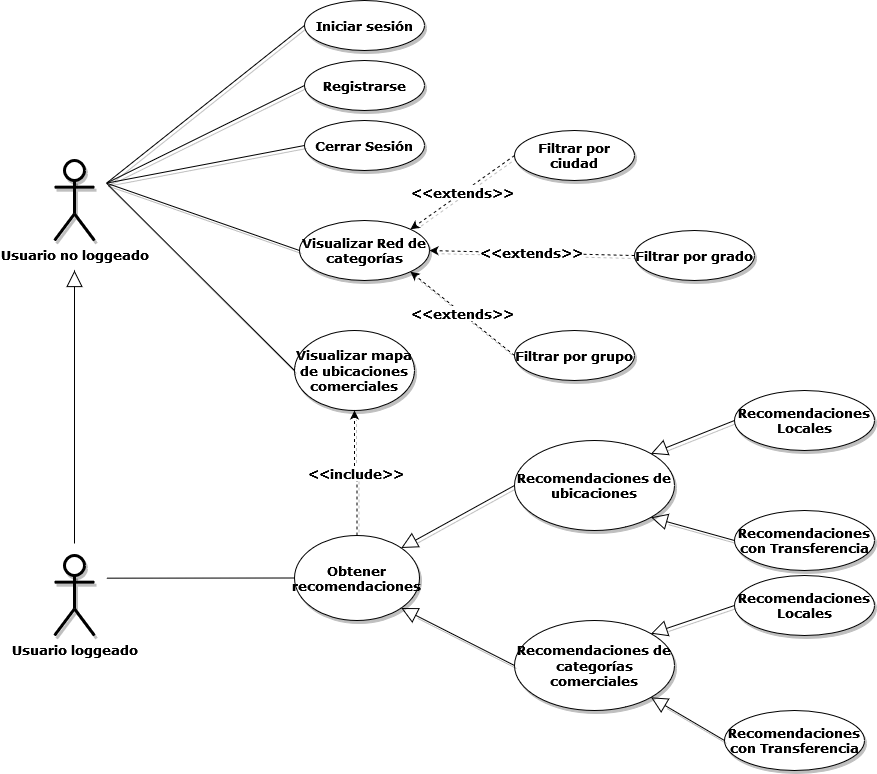
\includegraphics[height=1\textheight]{CasosDeUso}
	\caption{Casos de uso de la aplicación}\label{CasosDeUso}
\end{figure}
\FloatBarrier
%\imagen{CasosDeUso}{Casos de uso de la aplicación}

\end{landscape}


%Una muestra de cómo podría ser una tabla de casos de uso:
%
%% Caso de Uso 1 -> Consultar Experimentos.
%\begin{table}[p]
%	\centering
%	\begin{tabularx}{\linewidth}{ p{0.21\columnwidth} p{0.71\columnwidth} }
	%		\toprule
	%		\textbf{CU-1}    & \textbf{Ejemplo de caso de uso}\\
	%		\toprule
	%		\textbf{Versión}              & 1.0    \\
	%		\textbf{Autor}                & Alumno \\
	%		\textbf{Requisitos asociados} & RF-xx, RF-xx \\
	%		\textbf{Descripción}          & La descripción del CU \\
	%		\textbf{Precondición}         & Precondiciones (podría haber más de una) \\
	%		\textbf{Acciones}             &
	%		\begin{enumerate}
		%			\def\labelenumi{\arabic{enumi}.}
		%			\tightlist
		%			\item Pasos del CU
		%			\item Pasos del CU (añadir tantos como sean necesarios)
		%		\end{enumerate}\\
	%		\textbf{Postcondición}        & Postcondiciones (podría haber más de una) \\
	%		\textbf{Excepciones}          & Excepciones \\
	%		\textbf{Importancia}          & Alta o Media o Baja... \\
	%		\bottomrule
	%	\end{tabularx}
%	\caption{CU-1 Nombre del caso de uso.}
%\end{table}



\begin{table}[p]
	\centering
	\begin{tabularx}{\linewidth}{ p{0.21\columnwidth} p{0.71\columnwidth} }
			\toprule
			\textbf{CU-1}    & \textbf{Iniciar sesión}\\
			\toprule
			\textbf{Versión}              & 1.0    \\
			\textbf{Autor}                & Mario Hurtado \\
			\textbf{Requisitos asociados} & RF-7, RF-7.2, RF-1 \\
			\textbf{Descripción}          & Este caso de uso permite al usuario iniciar sesión con la cuenta con la que se había registrado. \\
			\textbf{Precondición}         & Contar con una cuenta ya registrada en la aplicación.\\
			\textbf{Acciones}             &
			\begin{enumerate}
					\def\labelenumi{\arabic{enumi}.}
					\tightlist
					\item Acceder a la página de inicio de sesión.
					\item Rellenar campo de nombre de usuario.
					\item Rellenar campo de contraseña.
					\item Pulsar en botón de inicio de sesión.
				\end{enumerate}\\
			\textbf{Postcondición}        & Redirección a la página de inicio con la sesión iniciada\\
			\textbf{Excepciones}          & Si el nombre o usuario no son válidos se muestra un mensaje de error. \\
			\textbf{Importancia}          & Alta\\
			\bottomrule
		\end{tabularx}
	\caption{CU-1 Inicio de sesión.}
\end{table}

%
%
\begin{table}[p]
	\centering
	\begin{tabularx}{\linewidth}{ p{0.21\columnwidth} p{0.71\columnwidth} }
			\toprule
			\textbf{CU-2}    & \textbf{Registro de usuario}\\
			\toprule
			\textbf{Versión}              & 1.0    \\
			\textbf{Autor}                & Mario Hurtado \\
			\textbf{Requisitos asociados} & RF-7, RF-7.1, RF-1 \\
			\textbf{Descripción}          & Este caso de uso permite al usuario registrar una cuenta en la aplicación. \\
			\textbf{Precondición}         & Acceder a la página de registro.\\
			\textbf{Acciones}             &
			\begin{enumerate}
					\def\labelenumi{\arabic{enumi}.}
					\tightlist
					\item Rellenar campo de nombre de usuario.
					\item Rellenar campo de nombre.
					\item Rellenar campo de apellido.
					\item Rellenar campo de correo electrónico.
					\item Rellenar campo de contraseña.
					\item Rellenar campo de repetir contraseña
				\end{enumerate}\\
			\textbf{Postcondición}        & \begin{itemize}
				\item Redirección a página de inicio.
				\item Sesión iniciada.
				\item Cuenta registrada en la base de datos.
			\end{itemize} \\
			\textbf{Excepciones}          & Mensaje de error en caso de que uno de los campos no sea válido o el usuario ya exista. \\
			\textbf{Importancia}          & Alta\\
			\bottomrule
		\end{tabularx}
	\caption{CU-2 Registro de usuario.}
\end{table}
%
%%% Caso de Uso 1 -> Consultar Experimentos.
\begin{table}[p]
	\centering
	\begin{tabularx}{\linewidth}{ p{0.21\columnwidth} p{0.71\columnwidth} }
			\toprule
			\textbf{CU-3}    & \textbf{Cierre de sesión}\\
			\toprule
			\textbf{Versión}              & 1.0    \\
			\textbf{Autor}                & Mario Hurtado \\
			\textbf{Requisitos asociados} & RF-7, RF-7.3, RF-1 \\
			\textbf{Descripción}          & Este caso de uso permite al usuario cerrar su sesión. \\
			\textbf{Precondición}         &  Sesión de usuario activa.\\
			\textbf{Acciones}             &
			\begin{enumerate}
					\def\labelenumi{\arabic{enumi}.}
					\tightlist
					\item Pulsar sobre el botón de cierre de sesión
				\end{enumerate}\\
			\textbf{Postcondición}        &  \begin{itemize}
				\item Sesión de usuario cerrada.
				\item Redirección a página de inicio.
			\end{itemize} \\
			\textbf{Excepciones}          & - \\
			\textbf{Importancia}          & Alta \\
			\bottomrule
		\end{tabularx}
	\caption{CU-3 Cierre de sesión de usuario.}
\end{table}
%
%%% Caso de Uso 1 -> Consultar Experimentos.
\begin{table}[p]
	\centering
	\begin{tabularx}{\linewidth}{ p{0.21\columnwidth} p{0.71\columnwidth} }
			\toprule
			\textbf{CU-4}    & \textbf{Visualizar red de categorías.}\\
			\toprule
			\textbf{Versión}              & 1.0    \\
			\textbf{Autor}                & Mario Hurtado \\
			\textbf{Requisitos asociados} & RF-6, RF-6.1, RF-6.3, RF-1 \\
			\textbf{Descripción}          & Este caso de uso permite al usuario visualizar una red de interacción entre categorías. \\
			\textbf{Precondición}         &  - \\
			\textbf{Acciones}             &
			\begin{enumerate}
					\def\labelenumi{\arabic{enumi}.}
					\tightlist
					\item Pulsar en el botón de visualización de red.
				\end{enumerate}\\
			\textbf{Postcondición}        & Redirección a la página de visualización de red de categorías.\\
			\textbf{Excepciones}          &  - \\
			\textbf{Importancia}          & Media \\
			\textbf{Puntos de ampliación} & CU-5, CU-6, CU-7\\
			
			\bottomrule
		\end{tabularx}
	\caption{CU-4 Visualizar red de categorías.}
\end{table}
%
%%% Caso de Uso 1 -> Consultar Experimentos.
\begin{table}[p]
	\centering
	\begin{tabularx}{\linewidth}{ p{0.21\columnwidth} p{0.71\columnwidth} }
			\toprule
			\textbf{CU-5}    & \textbf{Filtro por ciudad en visualización de red}\\
			\toprule
			\textbf{Versión}              & 1.0    \\
			\textbf{Autor}                & Mario Hurtado \\
			\textbf{Requisitos asociados} & RF-6, RF-6.1, RF-6.2, RF-1 \\
			\textbf{Descripción}          & Este caso de uso permite seleccionar de qué ciudad visualizar la red de categorías \\
			\textbf{Precondición}         & Encontrarse en la página de visualización de red\\
			\textbf{Acciones}             &
			\begin{enumerate}
					\def\labelenumi{\arabic{enumi}.}
					\tightlist
					\item El usuario abre el desplegable de ciudades y selecciona una
					\item El sistema hace una petición a la base de datos con la información de las categorías de la ciudad.
					\item La página visualiza la red de categorías.
				\end{enumerate}\\
			\textbf{Postcondición}        & Visualización de la red de categorías de la ciudad seleccionada \\
			\textbf{Excepciones}          & - \\
			\textbf{Importancia}          & Media \\
			\bottomrule
		\end{tabularx}
	\caption{CU-5 Filtro por ciudad en visualización de red.}
\end{table}
%
%%% Caso de Uso 1 -> Consultar Experimentos.
\begin{table}[p]
	\centering
	\begin{tabularx}{\linewidth}{ p{0.21\columnwidth} p{0.71\columnwidth} }
			\toprule
			\textbf{CU-6}    & \textbf{Filtro por grado en visualización de red}\\
			\toprule
			\textbf{Versión}              & 1.0    \\
			\textbf{Autor}                & Mario Hurtado \\
			\textbf{Requisitos asociados} & RF-6, RF-6.4, RF-1 \\
			\textbf{Descripción}          & Este caso de uso permite al usuario aplicar un filtro en base al grado de los nodos en la visualización de la red \\
			\textbf{Precondición}         & Ciudad seleccionada.\\
			\textbf{Acciones}             &
			\begin{enumerate}
					\def\labelenumi{\arabic{enumi}.}
					\tightlist
					\item El usuario selecciona un valor de grado.
					\item El sistema crea un subconjunto de nodos con aquellos con grado mayor o igual al seleccionado.
					\item El sistema actualiza la visualización de red.
				\end{enumerate}\\
			\textbf{Postcondición}        & Visualización de red actualizada con el filtro de grado.\\
			\textbf{Excepciones}          & - \\
			\textbf{Importancia}          & Media \\
			\bottomrule
		\end{tabularx}
	\caption{CU-6 Filtro por grado en visualización de red.}
\end{table}
%
%%% Caso de Uso 1 -> Consultar Experimentos.
\begin{table}[p]
	\centering
	\begin{tabularx}{\linewidth}{ p{0.21\columnwidth} p{0.71\columnwidth} }
			\toprule
			\textbf{CU-7}    & \textbf{Filtro por categoría en visualización de red}\\
			\toprule
			\textbf{Versión}              & 1.0    \\
			\textbf{Autor}                & Mario Hurtado \\
			\textbf{Requisitos asociados} & RF-6, RF-6.5, RF-1 \\
			\textbf{Descripción}          & Este caso de uso permite al usuario filtrar en base a la categoría de los nodos de la visualización de red\\
			\textbf{Precondición}         & Ciudad seleccionada en la visualización de red\\
			\textbf{Acciones}             &
			\begin{enumerate}
					\def\labelenumi{\arabic{enumi}.}
					\tightlist
					\item El usuario selecciona los categoría que desea ver.
					\item El sistema crea un subconjunto con los nodos que se encuentran dentro de las categorías seleccionadas por el usuario.
					\item El sistema reinicia el valor del filtro de grado.
					\item El sistema actualiza la visualización de la red.
				\end{enumerate}\\
			\textbf{Postcondición}        & Visualización de la red actualizada con el filtro de categoría\\
			\textbf{Excepciones}          & - \\
			\textbf{Importancia}          & Media \\
			\bottomrule
		\end{tabularx}
	\caption{CU-7 Filtro por categoría en visualización de red.}
\end{table}

%% Caso de Uso 1 -> Consultar Experimentos.
\begin{table}[p]
	\centering
	\begin{tabularx}{\linewidth}{ p{0.21\columnwidth} p{0.71\columnwidth} }
			\toprule
			\textbf{CU-8}    & \textbf{Visualizar mapa de ubicaciones comerciales}\\
			\toprule
			\textbf{Versión}              & 1.0    \\
			\textbf{Autor}                & Mario Hurtado \\
			\textbf{Requisitos asociados} & RF-3, RF-3.1, RF-3.6, RF-2, RF-1 \\
			\textbf{Descripción}          & Este caso de uso permite a los usuarios visualizar los establecimientos comerciales de distintas categorías en distintas ciudades \\
			\textbf{Precondición}         & -\\
			\textbf{Acciones}             &
			\begin{enumerate}
					\def\labelenumi{\arabic{enumi}.}
					\tightlist
					\item El usuario selecciona una ciudad.
					\item El sistema carga en el menú las categorías comerciales disponibles para la ciudad seleccionada.
					\item El usuario selecciona una categoría comercial.
					\item El sistema sitúa el mapa en las coordenadas de la ciudad.
					\item El sistema muestra los marcadores con los establecimientos comerciales en el mapa
				\end{enumerate}\\
			\textbf{Postcondición}        & Mapa situado en las coordenadas de la ciudad seleccionada y con los marcadores correspondientes a la categoría elegida.\\
			\textbf{Excepciones}          & - \\
			\textbf{Importancia}          & Alta \\
			\bottomrule
		\end{tabularx}
	\caption{CU-8 Visualizar mapa de ubicaciones comerciales.}
\end{table}

%% Caso de Uso 1 -> Consultar Experimentos.
\begin{table}[p]
	\centering
	\begin{tabularx}{\linewidth}{ p{0.21\columnwidth} p{0.71\columnwidth} }
			\toprule
			\textbf{CU-9}    & \textbf{Recomendaciones de ubicaciones a nivel local}\\
			\toprule
			\textbf{Versión}              & 1.0    \\
			\textbf{Autor}                & Mario Hurtado \\
			\textbf{Requisitos asociados} & RF-3, RF-3.2, RF3.4, RF-3.5, RF-3.6, RF-3.7, RF-3.8, RF-5, RF-5.1, RF-1  \\
			\textbf{Descripción}          & Este caso de uso permite al usuario obtener recomendaciones a nivel local en base a ubicaciones que haya seleccionado\\
			\textbf{Precondición}         & \begin{itemize}
							\tightlist
				\item Usuario con sesión iniciada.
				\item Encontrarse en la página del mapa.
				\end{itemize}\\
			\textbf{Acciones}             &
			\begin{enumerate}
					\def\labelenumi{\arabic{enumi}.}
					\tightlist
					\item El usuario selecciona los establecimientos y ubicaciones en los que está interesado
					\item El usuario pulsa el botón de recomendaciones de ubicaciones a nivel local.
					\item El sistema redirige a la página de recomendaciones a nivel local, mostrando en el mapa las ubicaciones seleccionadas con un identificador.
					\item El sistema calcula los valores para las recomendaciones.
					\item El usuario selecciona la categoría comercial en la que está interesado.
					\item El usuario selecciona el método a emplear.
					\item El sistema muestra las ubicaciones seleccionadas ordenadas en orden descendente según la adecuación a la categoría seleccionada.
				\end{enumerate}\\
			\textbf{Postcondición}        & Resultados de recomendaciones de ubicaciones. Orden descendente según adecuación a la categoría seleccionada\\
			\textbf{Incluye}   & CU-8\\
			\textbf{Excepciones}          & - \\
			\textbf{Importancia}          & Alta  \\
			\bottomrule
		\end{tabularx}
	\caption{CU-9 Recomendaciones de ubicaciones a nivel local.}
\end{table}

\begin{table}[p]
	\centering
	\begin{tabularx}{\linewidth}{ p{0.21\columnwidth} p{0.71\columnwidth} }
		\toprule
		\textbf{CU-10}    & \textbf{Recomendaciones de ubicaciones con transferencia}\\
		\toprule
		\textbf{Versión}              & 1.0    \\
		\textbf{Autor}                & Mario Hurtado \\
		\textbf{Requisitos asociados} & RF-3, RF-3.2, RF3.4, RF-3.5, RF-3.6, RF-3.7, RF-3.8, RF-5, RF-5.2, RF-1  \\
		\textbf{Descripción}          & Este caso de uso permite al usuario obtener recomendaciones en base a ubicaciones que haya seleccionado empleando transferencia de conocimiento.\\
		\textbf{Precondición}         & \begin{itemize}
						\tightlist
			\item Usuario con sesión iniciada.
			\item Encontrarse en la página del mapa.
		\end{itemize}\\
		\textbf{Acciones}             &
		\begin{enumerate}
			\def\labelenumi{\arabic{enumi}.}
			\tightlist
			\item El usuario selecciona los establecimientos y ubicaciones en los que está interesado
			\item El usuario pulsa el botón de recomendaciones de ubicaciones con transferencia.
			\item El sistema redirige a la página de recomendaciones con transferencia, mostrando en el mapa las ubicaciones seleccionadas con un identificador.
			\item El usuario selecciona una ciudad.
			\item El sistema actualiza las categorías disponibles
			\item El sistema calcula los valores para las recomendaciones.
			\item El usuario selecciona la categoría comercial en la que está interesado.
			\item El usuario selecciona el método a emplear.
			\item El sistema muestra las ubicaciones seleccionadas ordenadas en orden descendente según la adecuación a la categoría seleccionada.
		\end{enumerate}\\
		\textbf{Postcondición}        & Resultados de recomendaciones de ubicaciones. Orden descendente según adecuación a la categoría seleccionada\\
		\textbf{Incluye}   & CU-8\\
		\textbf{Excepciones}          & - \\
		\textbf{Importancia}          & Alta  \\
		\bottomrule
	\end{tabularx}
	\caption{CU-10 Recomendaciones de ubicaciones con transferencia.}
\end{table}

\begin{table}[p]
	\centering
	\begin{tabularx}{\linewidth}{ p{0.21\columnwidth} p{0.71\columnwidth} }
		\toprule
		\textbf{CU-11}    & \textbf{Recomendaciones de categorías a nivel local}\\
		\toprule
		\textbf{Versión}              & 1.0    \\
		\textbf{Autor}                & Mario Hurtado \\
		\textbf{Requisitos asociados} & RF-3, RF-3.2, RF3.4, RF-3.5, RF-3.6, RF-3.7, RF-3.8, RF-4, RF-4.1, RF-1  \\
		\textbf{Descripción}          & Este caso de uso permite al usuario obtener recomendaciones de categorías en base a las ubicaciones que haya seleccionado a nivel local.\\
		\textbf{Precondición}         & \begin{itemize}
						\tightlist
			\item Usuario con sesión iniciada.
			\item Encontrarse en la página del mapa.
		\end{itemize}\\
		\textbf{Acciones}             &
		\begin{enumerate}
			\def\labelenumi{\arabic{enumi}.}
			\tightlist
			\item El usuario selecciona los establecimientos y ubicaciones en los que está interesado
			\item El usuario pulsa el botón de recomendaciones de categorías a nivel local.
			\item El sistema redirige a la página de recomendaciones de categorías a nivel local, mostrando en el mapa las ubicaciones seleccionadas con un identificador.
			\item El sistema calcula los valores para las recomendaciones.
			\item El usuario selecciona el método a emplear.
			\item El sistema muestra las ubicaciones seleccionadas junto con las categorías comerciales más adecuadas para cada una.
		\end{enumerate}\\
		\textbf{Postcondición}        & Resultados de recomendaciones de categorías para cada ubicación\\
		\textbf{Incluye}   & CU-8\\
		\textbf{Excepciones}          & - \\
		\textbf{Importancia}          & Alta  \\
		\bottomrule
	\end{tabularx}
	\caption{CU-11 Recomendaciones de categorías a nivel local.}
\end{table}


\begin{table}[p]
	\centering
	\begin{tabularx}{\linewidth}{ p{0.21\columnwidth} p{0.71\columnwidth} }
		\toprule
		\textbf{CU-12}    & \textbf{Recomendaciones de categorías con transferencia}\\
		\toprule
		\textbf{Versión}              & 1.0    \\
		\textbf{Autor}                & Mario Hurtado \\
		\textbf{Requisitos asociados} & RF-3, RF-3.2, RF3.4, RF-3.5, RF-3.6, RF-3.7, RF-3.8, RF-4, RF-4.2, RF-1  \\
		\textbf{Descripción}          & Este caso de uso permite al usuario obtener recomendaciones de categorías en base a las ubicaciones que haya seleccionado empleando transferencia.\\
		\textbf{Precondición}         & \begin{itemize}
			\tightlist
			\item Usuario con sesión iniciada.
			\item Encontrarse en la página del mapa.
		\end{itemize}\\
		\textbf{Acciones}             &
		\begin{enumerate}
			\def\labelenumi{\arabic{enumi}.}
			\tightlist
			\item El usuario selecciona los establecimientos y ubicaciones en los que está interesado
			\item El usuario pulsa el botón de recomendaciones de categorías con transferencia.
			\item El sistema redirige a la página de recomendaciones de categorías con transferencia, mostrando en el mapa las ubicaciones seleccionadas con un identificador.
			\item El usuario selecciona una ciudad.
			\item El sistema calcula las recomendaciones.
			\item El usuario selecciona el método a emplear.
			\item El sistema muestra las ubicaciones seleccionadas junto con las categorías comerciales más adecuadas para cada una.
		\end{enumerate}\\
		\textbf{Postcondición}        & Resultados de recomendaciones de categorías para cada ubicación según la ciudad seleccionada.\\
		\textbf{Incluye}   & CU-8\\
		\textbf{Excepciones}          & - \\
		\textbf{Importancia}          & Alta  \\
		\bottomrule
	\end{tabularx}
	\caption{CU-12 Recomendaciones de categorías con transferencia.}
\end{table}